\documentclass[a4paper, 12pt]{article}

\usepackage{babel}
\usepackage{enumitem}
\usepackage{times}
\usepackage{graphicx}
\usepackage{geometry}
	\geometry{left = 3cm, top = 3cm, right = 3cm, bottom = 3cm}
\usepackage{float}
\usepackage{setspace}
	\setstretch{1.5}
\usepackage{listings}


\begin{document}
\title{\huge\textbf{TUGAS BESAR DATABASE II}}
\date{18 DESEMBER 2019}

\maketitle


\begin{figure}[!ht]
\begin{center}

\includegraphics[width = 7cm, height = 7cm]{figure/P.jpg}
\end{center}
\end{figure}

\begin{center}
Disusun oleh :\\
JOHN KEVIN GIRALDI\\
D4 TI 2C\\
1.18.4.049\\
\vspace{1cm}
\textbf{PROGRAM DIPLOMA IV POLITEKNIK POS INDONESIA} \linebreak
\textbf{POLITEKNIK POS INDONESIA} \linebreak
\textbf{BANDUNG}\linebreak
\textbf{2019}
\end{center}

\section{PROSES PEMBUATAN TABEL}
\begin{enumerate}
\item Pertama kita harus membuka website
https://apex.oracle.com/pls/apex/f?p=4550:1:712758
388074636::::: untuk melakukan \textit{login} disini saya menggunakan akun dan \textit{workspace} yang telah saya buat : \\
\textit{Workspace}  : APEX\textunderscore KEVIN \\
\textit{Username}   : johnkevin1305@gmail.com \\
\textit{Password}   : johnkev12 \\
Link aplikasi       : 
https://apex.oracle.com/pls/apex/f?p=70162:7:110993318567207::NO:::
\begin{figure}[h]
\begin{center}
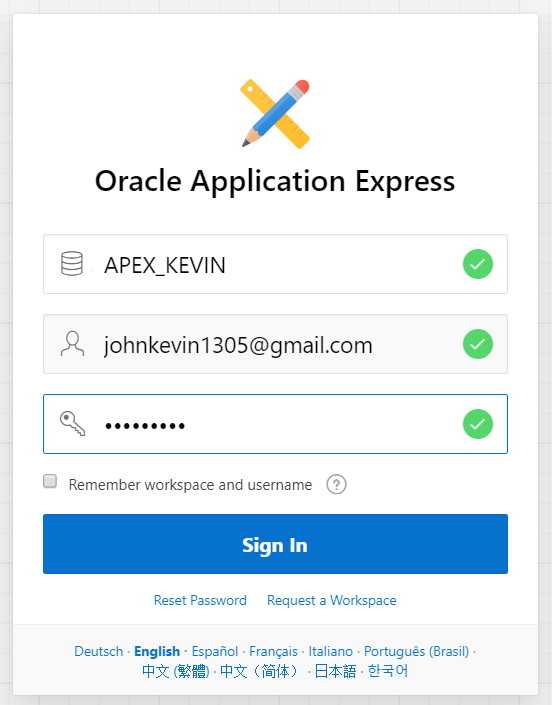
\includegraphics[width=5cm]{figure/Login.png}
\caption{Login}
\end{center}
\end{figure}

\item Setelah melakukan \textit{login} maka akan muncul tampilan yang terdiri dari berubah ke halaman utama \textit{Oracle Apex} seperti ini:

\begin{figure}[h]
\begin{center}
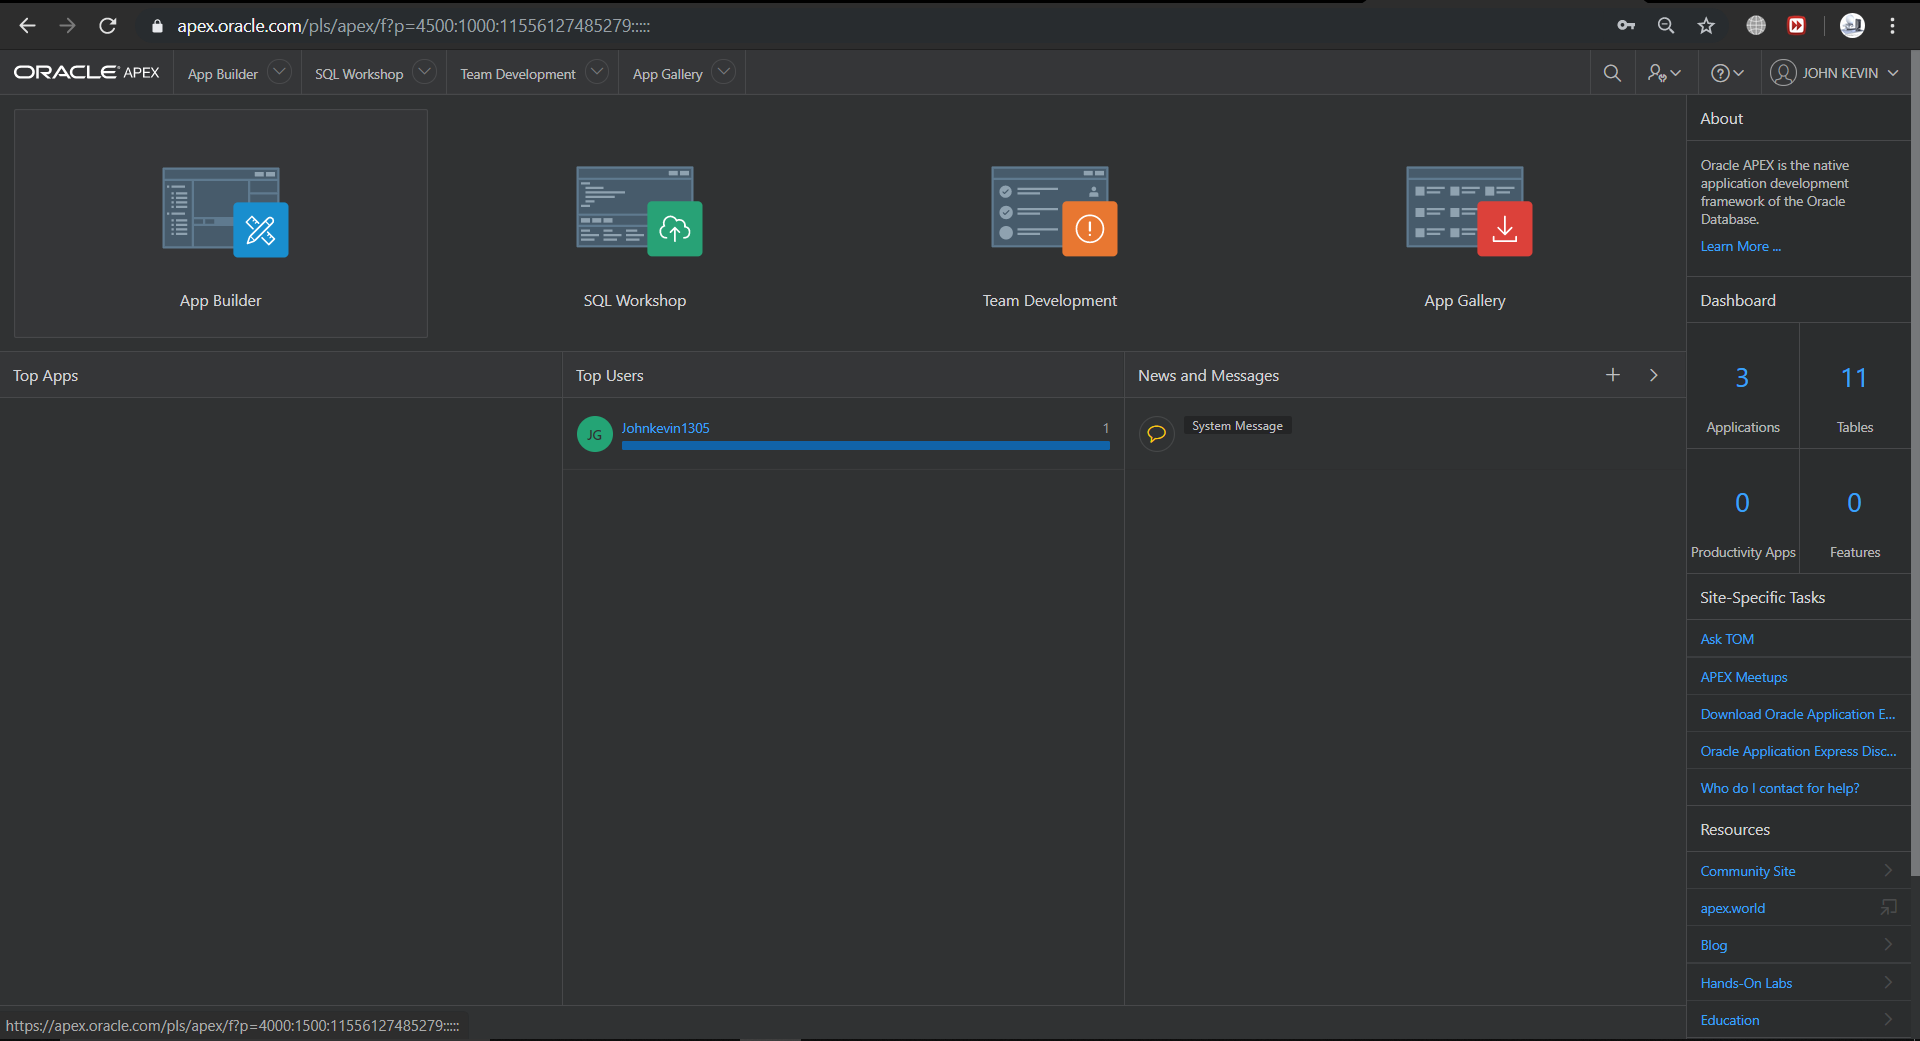
\includegraphics[width=7cm]{figure/T.png}
\caption{HALAMAN UTAMA ORACLE APEX}
\end{center}
\end{figure}

\item Lalu pilih \textit{SQL Command} pada \textit{SQL Workshop} untuk menuju ke halaman pengkodean atau \textit{query}.
\begin{figure}[h]
\begin{center}
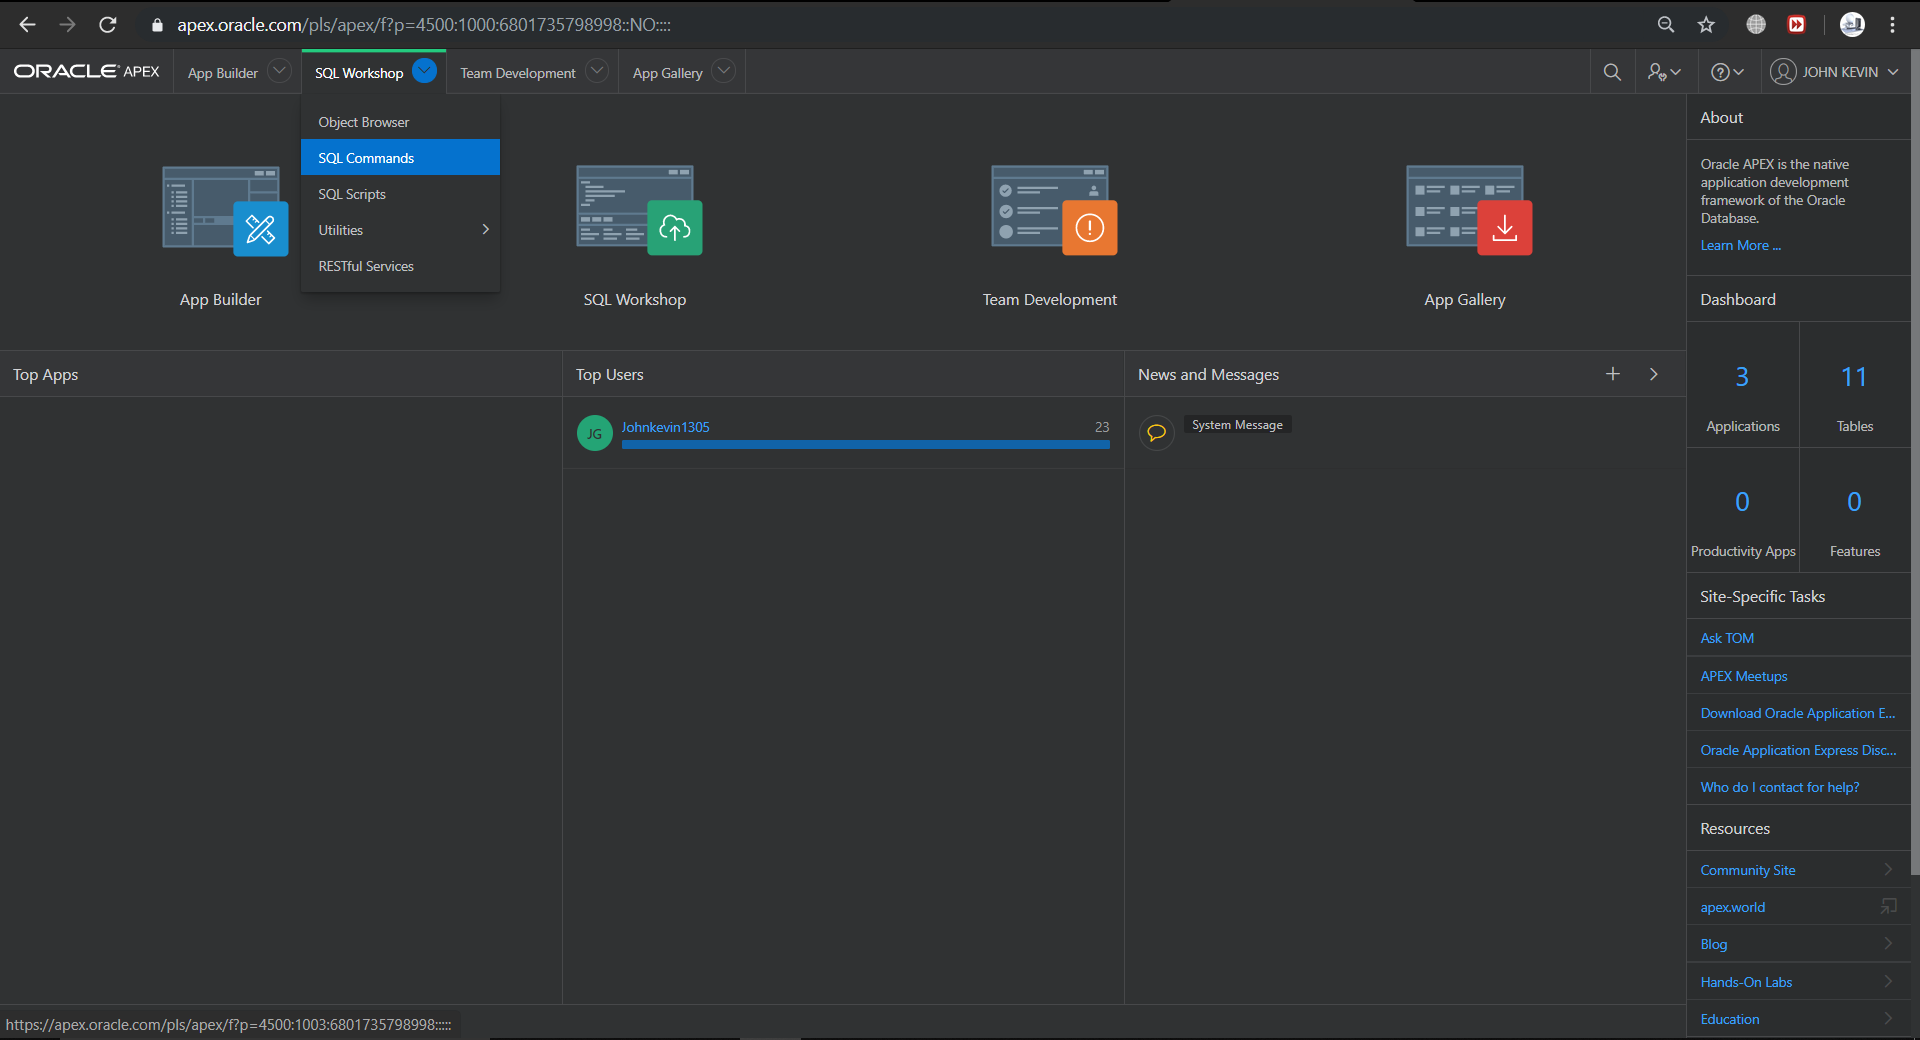
\includegraphics[width=12cm]{figure/SC.png}
\caption{SQL WORKSHOP}
\end{center}
\end{figure}

\item Setelah muncul halaman pengkodean, sekarang kita akan mulai membuat \textit{query} untuk membentuk tabel-tabel yang kita inginkan. Disini saya akan membuat 6 tabel yang terdiri dari:
\begin{itemize}
    \item PASIEN dengan \textit{Primary Key} (ID\textunderscore PASIEN)
    \item OBAT dengan \textit{Primary Key} (ID\textunderscore OBAT)
    \item DOKTER dengan \textit{Primary Key} (ID\textunderscore DOKTER)
    \item DIAGNOSA dengan \textit{Primary Key} (ID\textunderscore DIAGNOSA) yang berelasi dengan tabel PASIEN, DOKTER dan RESEP yang membentuk beberapa FK/\textit{Foreign Key} dari setiap relasi yang di hasilkan. \textit{Foreign Key}(ID\textunderscore PASIEN \textunderscore FK), \textit{Foreign Key} (ID\textunderscore DOKTER \textunderscore FK), \textit{Foreign Key} (ID\textunderscore RESEP \textunderscore FK).
    \item RESEP dengan \textit{Primary Key} (ID\textunderscore RESEP) yang berelasi dengan tabel OBAT, PASIEN DAN DOKTER yang membentuk beberapa FK/\textit{Foreign Key} dari setiap relasi yang di hasilkan. \textit{Foreign Key}(ID\textunderscore OBAT \textunderscore FK), \textit{Foreign Key} (ID\textunderscore PASIEN2 \textunderscore FK), \textit{Foreign Key} (ID\textunderscore DOKTER2 \textunderscore FK).
    \item LOG\textunderscore PASIEN tanpa \textit{Primary Key} ataupun \textit{Foreign Key}
\end{itemize}
\begin{figure}[h]
\begin{center}
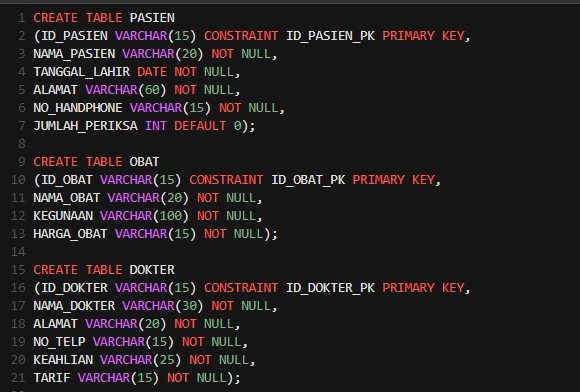
\includegraphics[width=7cm]{figure/CT1.png}
\caption{PEMBUATAN TABEL}
\end{center}
\end{figure}
\begin{figure}[h]
\begin{center}
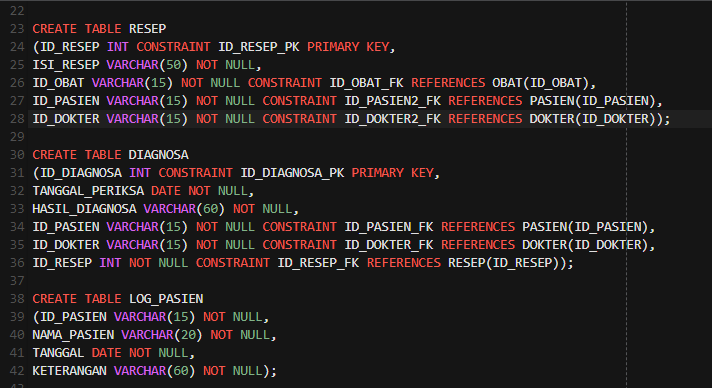
\includegraphics[width=7cm]{figure/CT2.png}
\caption{PEMBUATAN TABEL}
\end{center}
\end{figure}

\item Setelah kita berhasil membuat tabel-tabel yang diinginkan, selanjutnya kita akan menyisipkan data pada tabel PASIEN, DOKTER, OBAT, RESEP, DIAGNOSA, LOG\textunderscore PASIEN
\begin{figure}[h]
\begin{center}
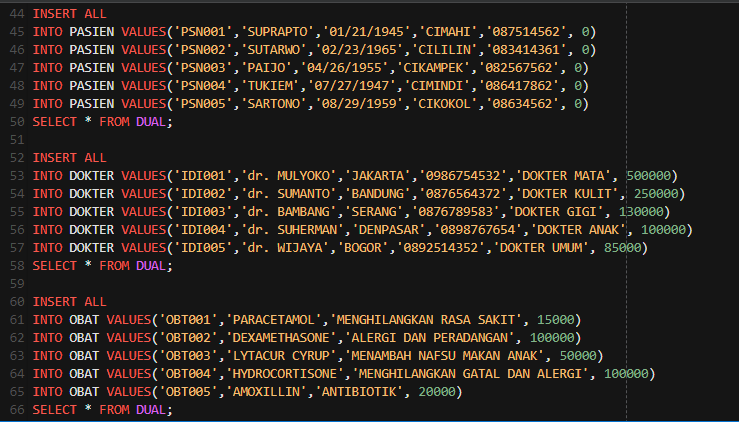
\includegraphics[width=7cm]{figure/I1.png}
\caption{MENYISIPKAN DATA}
\end{center}
\end{figure}

Sebelum menyisipkan data ke tabel berikutnya, kita harus membuat \textit{sequnce} terlebih dahulu, untuk mengaktifkan kode yang dirancang dan membuat penomoran secara otomatis atau \textit{auto increment}.
\begin{figure}[h]
\begin{center}
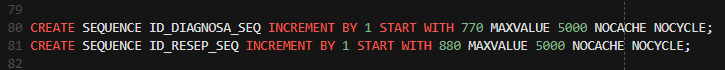
\includegraphics[width=7cm]{figure/SQ.png}
\caption{MEMBUAT SEQUENCE}
\end{center}
\end{figure}

Setelah \textit{sequence} dibuat maka \textit{query} untuk menyisipkan data pada tabel RESEP dan DIAGNOSA dapat digunakan.
\begin{figure}[h]
\begin{center}
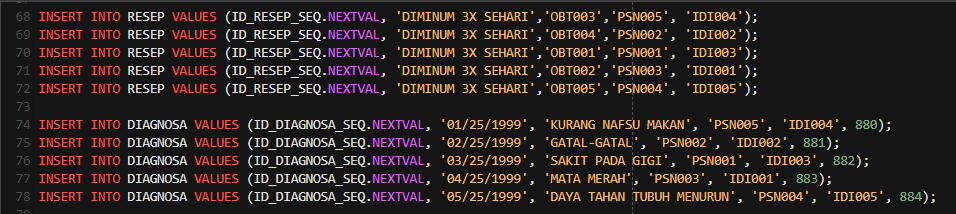
\includegraphics[width=8cm]{figure/I2.png}
\caption{MENYISIPKAN DATA}
\end{center}
\end{figure}

Mengapa saya tidak menyisipkan data pada tabel LOG\textunderscore PASIEN? Karena tabel ini saya gunakan untuk penyimpanan data secara otomatis jika proses \textit{trigger} atau \textit{delete,update,insert} dilakukan langsung tercatat pada tabel LOG\textunderscore PASIEN. \\

\item Setelah semua data telah disisipkan pada setiap tabel, selanjutnya kita akan membuat \textit{trigger} untuk membuat sebuat skema agar kita mengetahui setiap data yang di \textit{insert,update} maupun \textit{delete} pada tabel yang sudah ditentukan atau ditandai dengan \textit{trigger} itu sendiri.
\begin{figure}[h]
\begin{center}
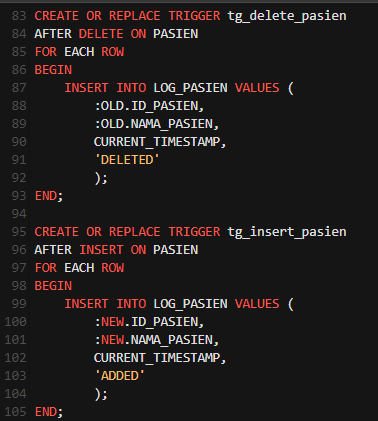
\includegraphics[width=6cm]{figure/TR1.png}
\caption{MEMBUAT TRIGGER}
\end{center}
\end{figure}
\begin{figure}[h]
\begin{center}
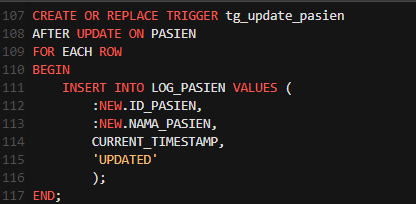
\includegraphics[width=6cm]{figure/TR2.png}
\caption{MEMBUAT TRIGGER}
\end{center}
\end{figure} \\

Cara mengecek \textit{trigger} yang telah dibuat: \\
Pilih \textit{Object Browser}
\begin{figure}[h]
\begin{center}
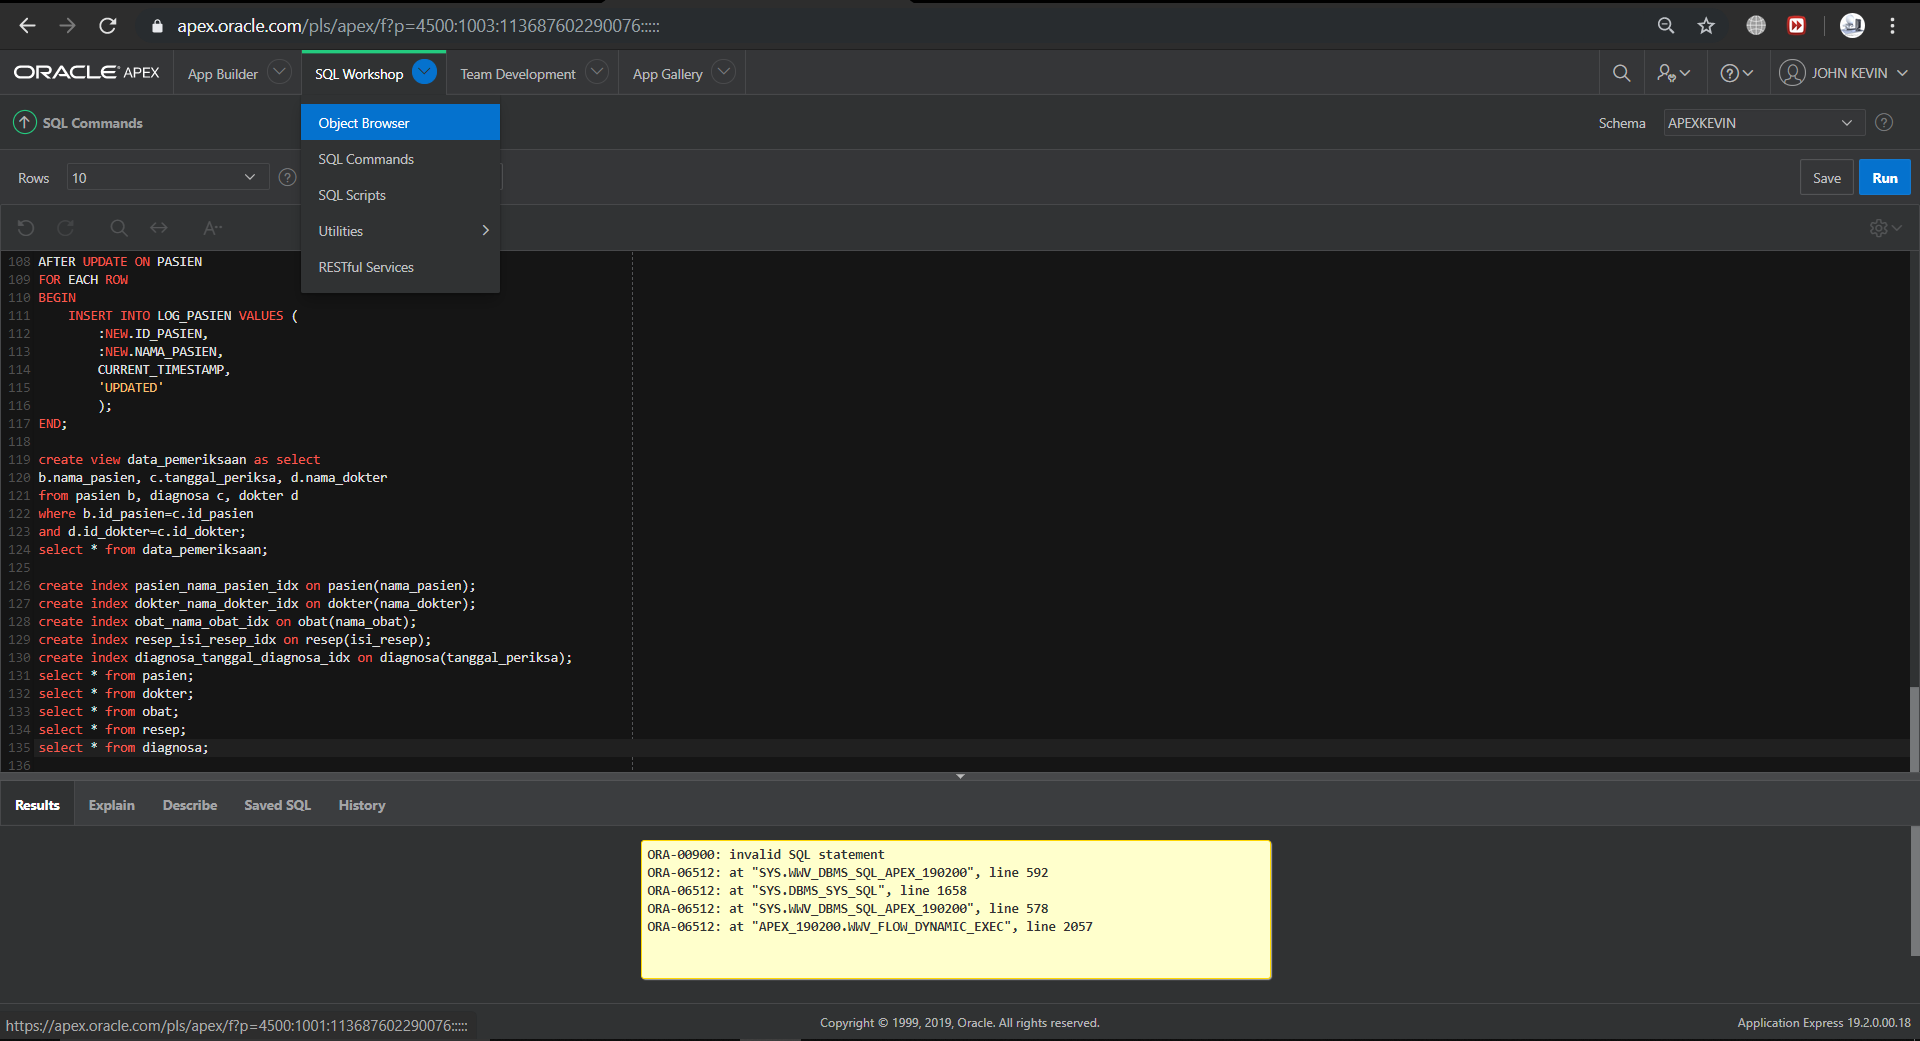
\includegraphics[width=6cm]{figure/OB.png}
\caption{OBJECT BROWSER}
\end{center}
\end{figure} \\

Lalu pilih \textit{trigger}
\begin{figure}[h]
\begin{center}
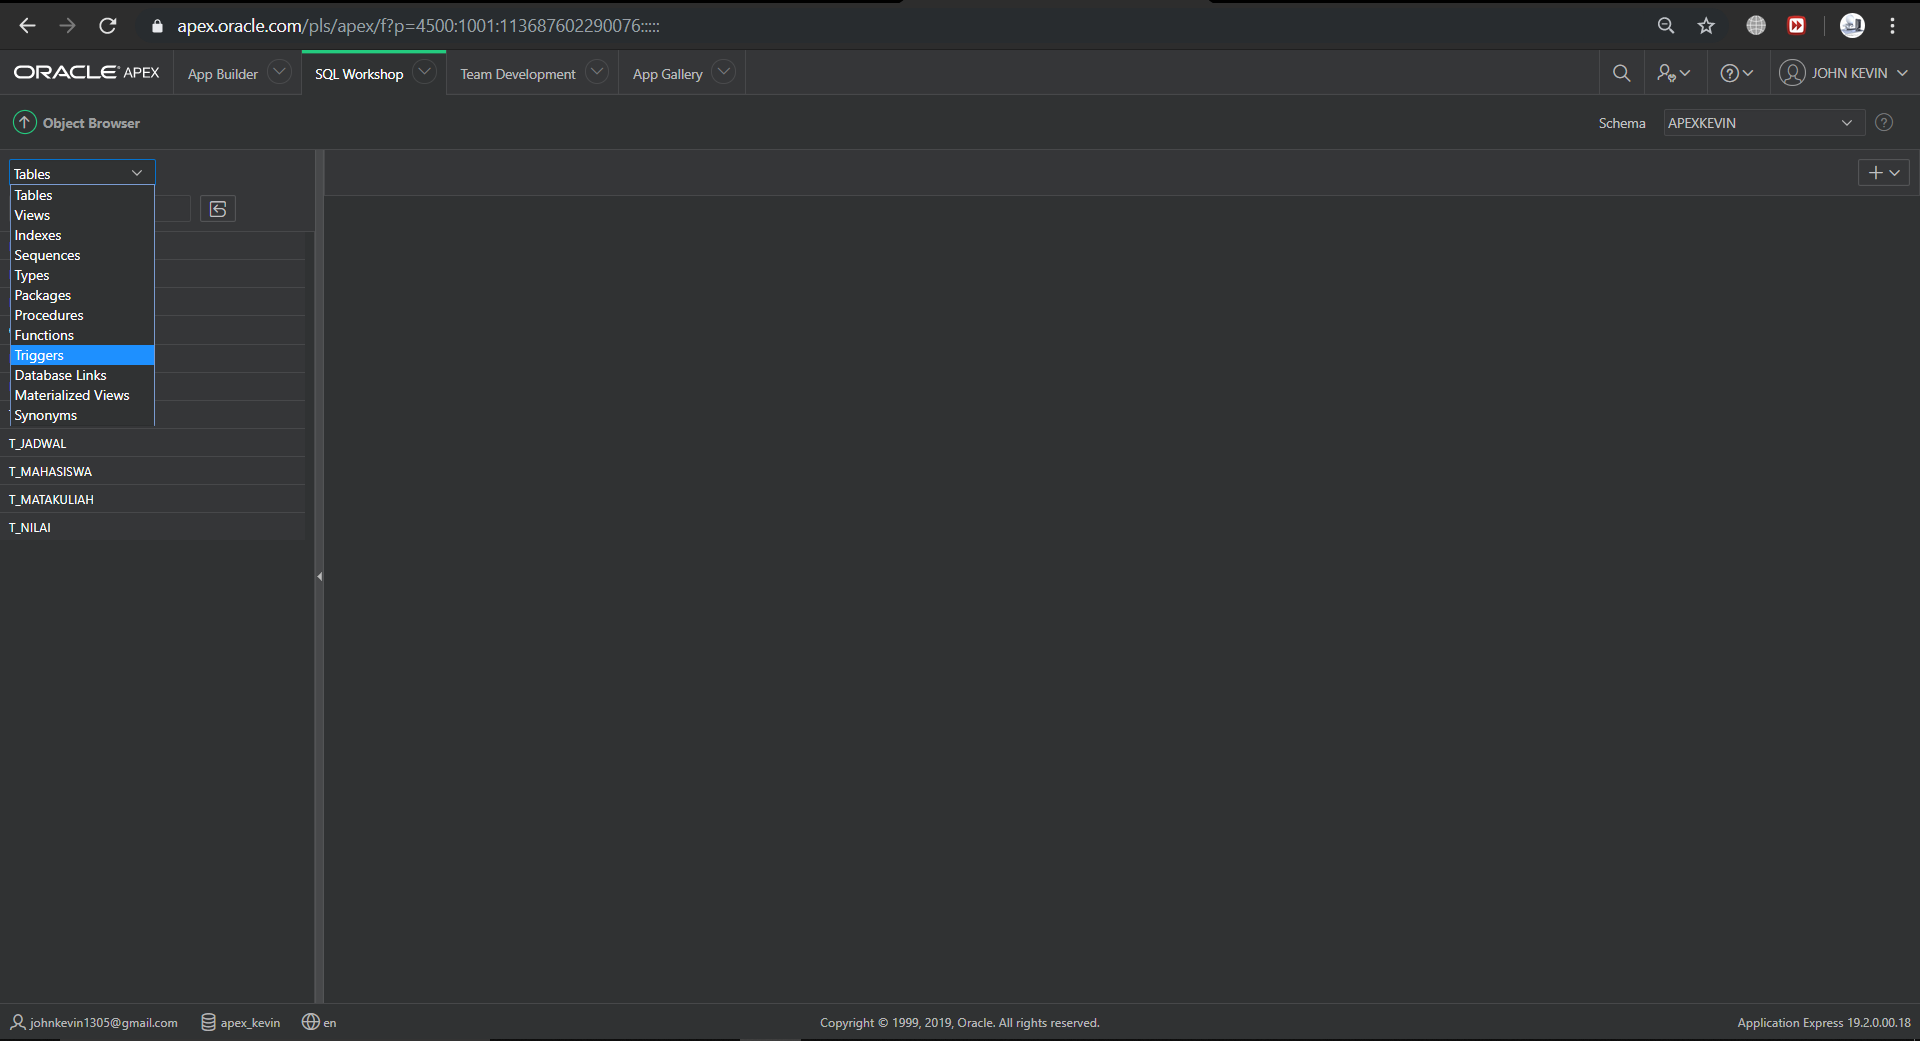
\includegraphics[width=6cm]{figure/TR.png}
\caption{TRIGGER}
\end{center}
\end{figure}

\item Selanjutnya kita akan membuat \textit{view} seperti yang kita tahu, \textit{view} digunakan untuk membuat sebuah tabel \textit{virtual} (bukan tabel sebenarnya) yang dibuat dari beberapa tabel lain. \textit{SQL View} tidak memiliki data sendiri, tetapi data-datanya berasal dari tabel-tabel atau yang telah ber\textit{korelasi}. \textit{View} digunakan untuk memudahkan atau menyederhanakan data yang ditampilkan.
\begin{figure}[h]
\begin{center}
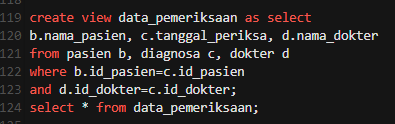
\includegraphics[width=9.25cm]{figure/V.png}
\caption{MEMBUAT VIEW}
\end{center}
\end{figure}
\end{enumerate}

Cara melihat menggunakan \textit{query} pada \textit{create view} yang telah dibuat: //
\begin{figure}[h]
\begin{center}
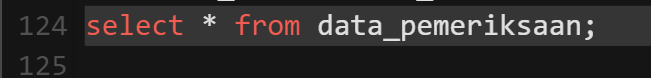
\includegraphics[width=9.25cm]{figure/CEK.png}
\caption{MELIHAT VIEW}
\end{center}
\end{figure}

\section{CREATE APLICATION}
Setelah proses query dalam pembuatan tabel dan penyisipan data selesai kita akan menuju ke pembuatan aplikasi. Langkah-langkah pembuatan aplikasi adalah sebagai berikut:
\begin{enumerate}
\item Pertama kita pilih \textit{Oracle Apex} (pada lingkaran\textunderscore biru) untuk menuju ke halaman utama
\begin{figure}[h]
\begin{center}
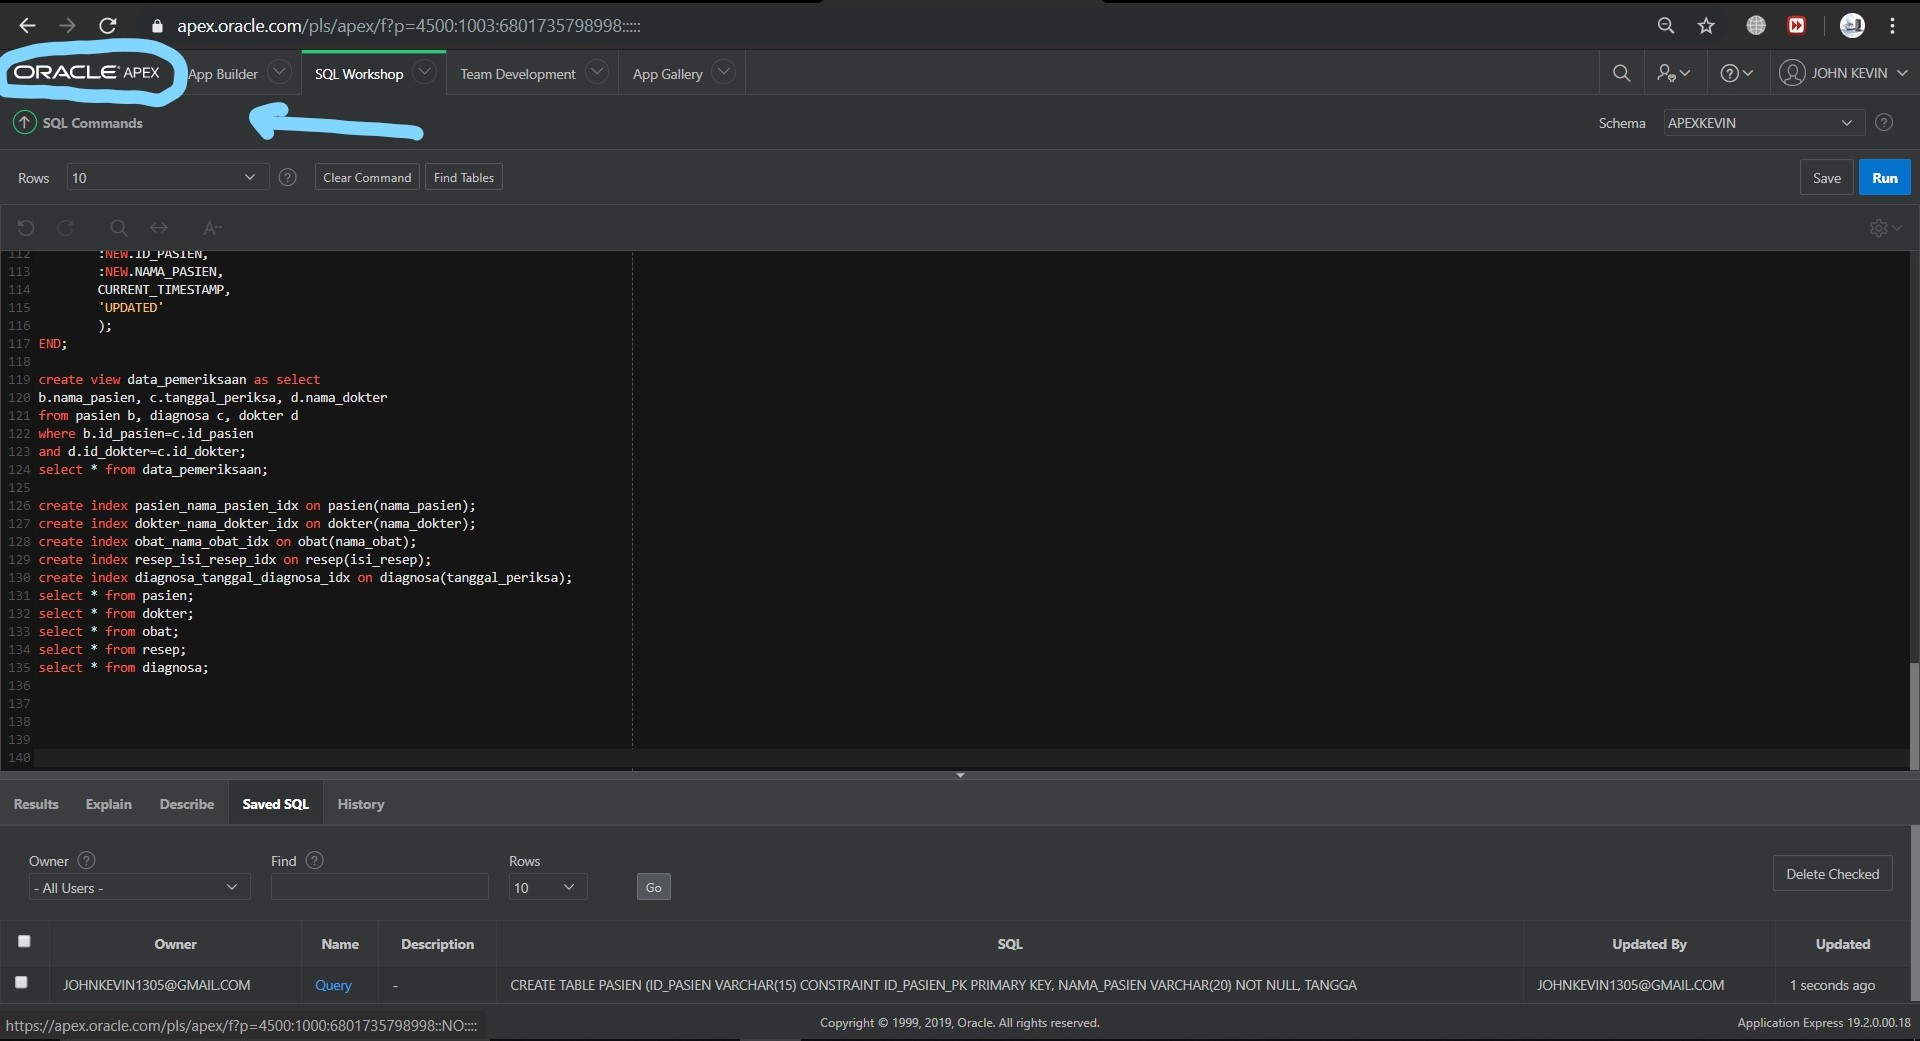
\includegraphics[width=10cm]{figure/H1.png}
\caption{MENUJU KE HALAMAN UTAMA}
\end{center}
\end{figure}

\item Lalu pilih \textit{App Builder}
\begin{figure}[h]
\begin{center}
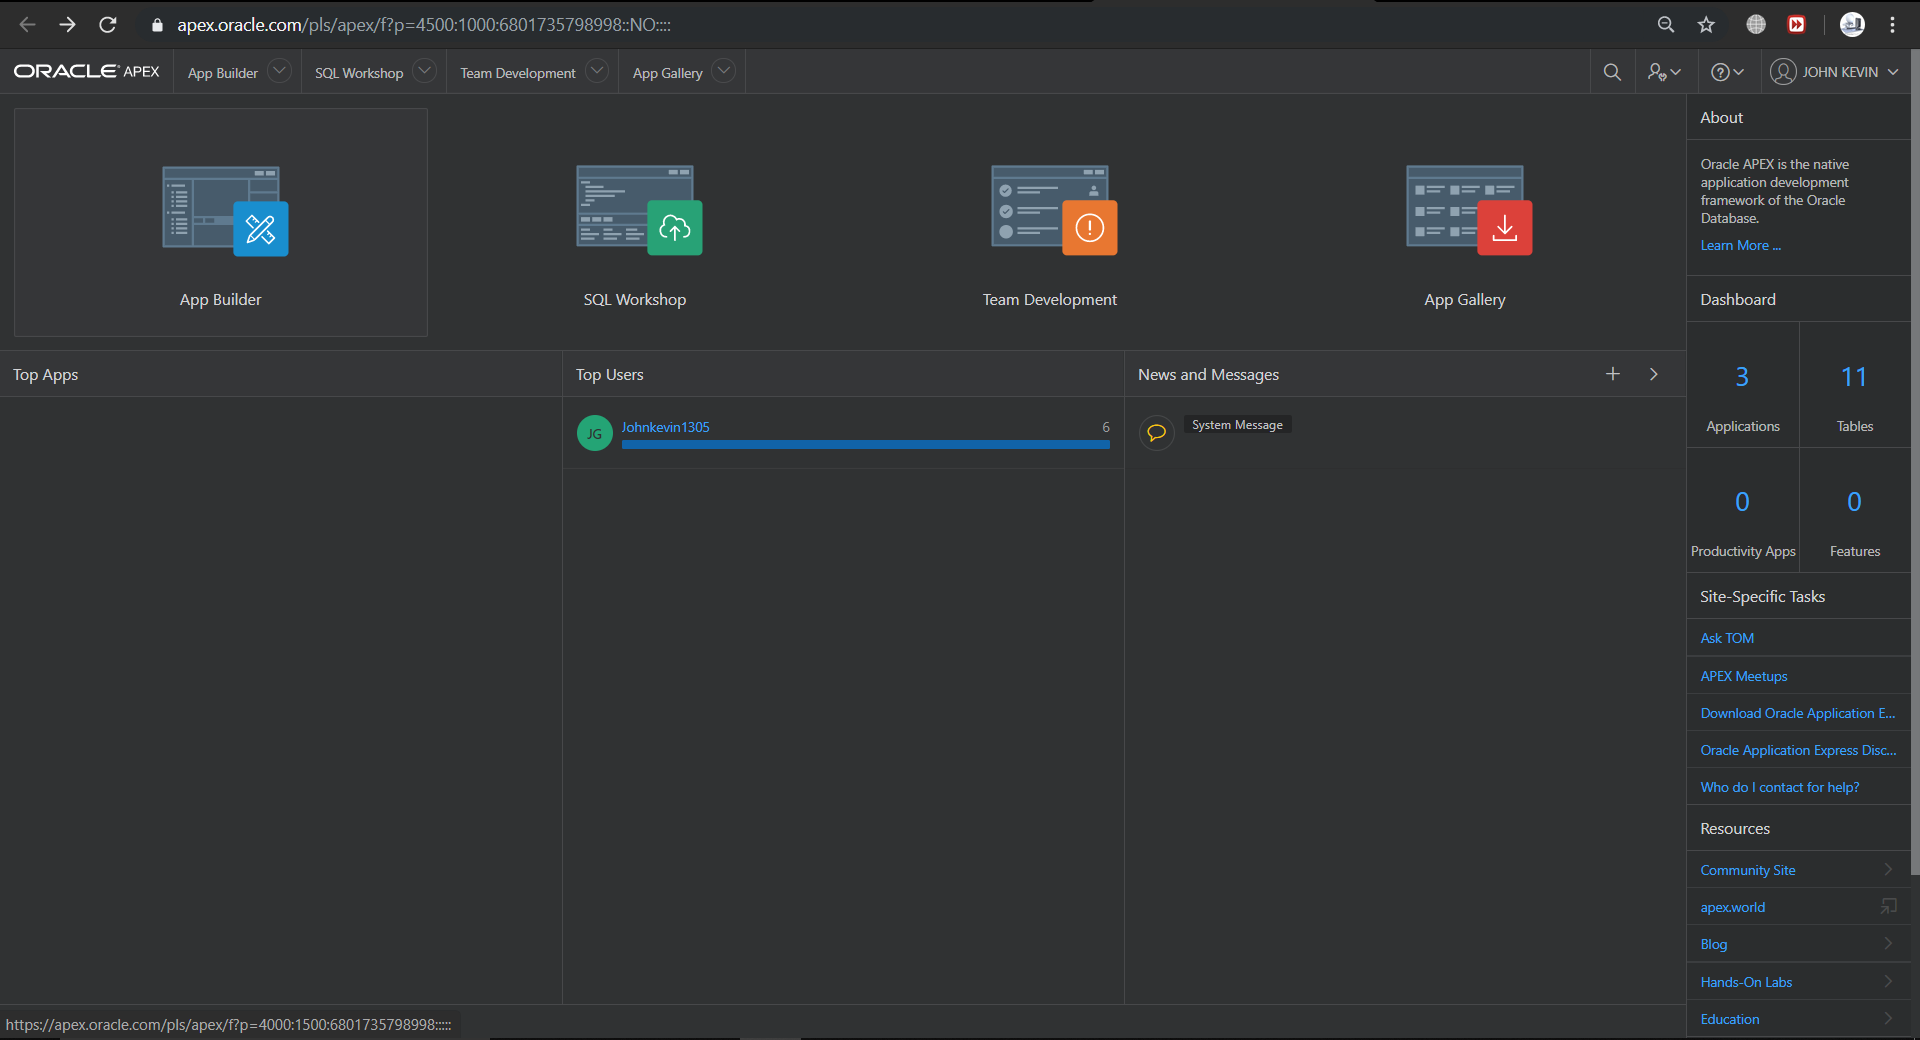
\includegraphics[width=8cm]{figure/AB.png}
\caption{APP BUILDER}
\end{center}
\end{figure}

\item Selanjutnya pilih \textit{Create}
\begin{figure}[h]
\begin{center}
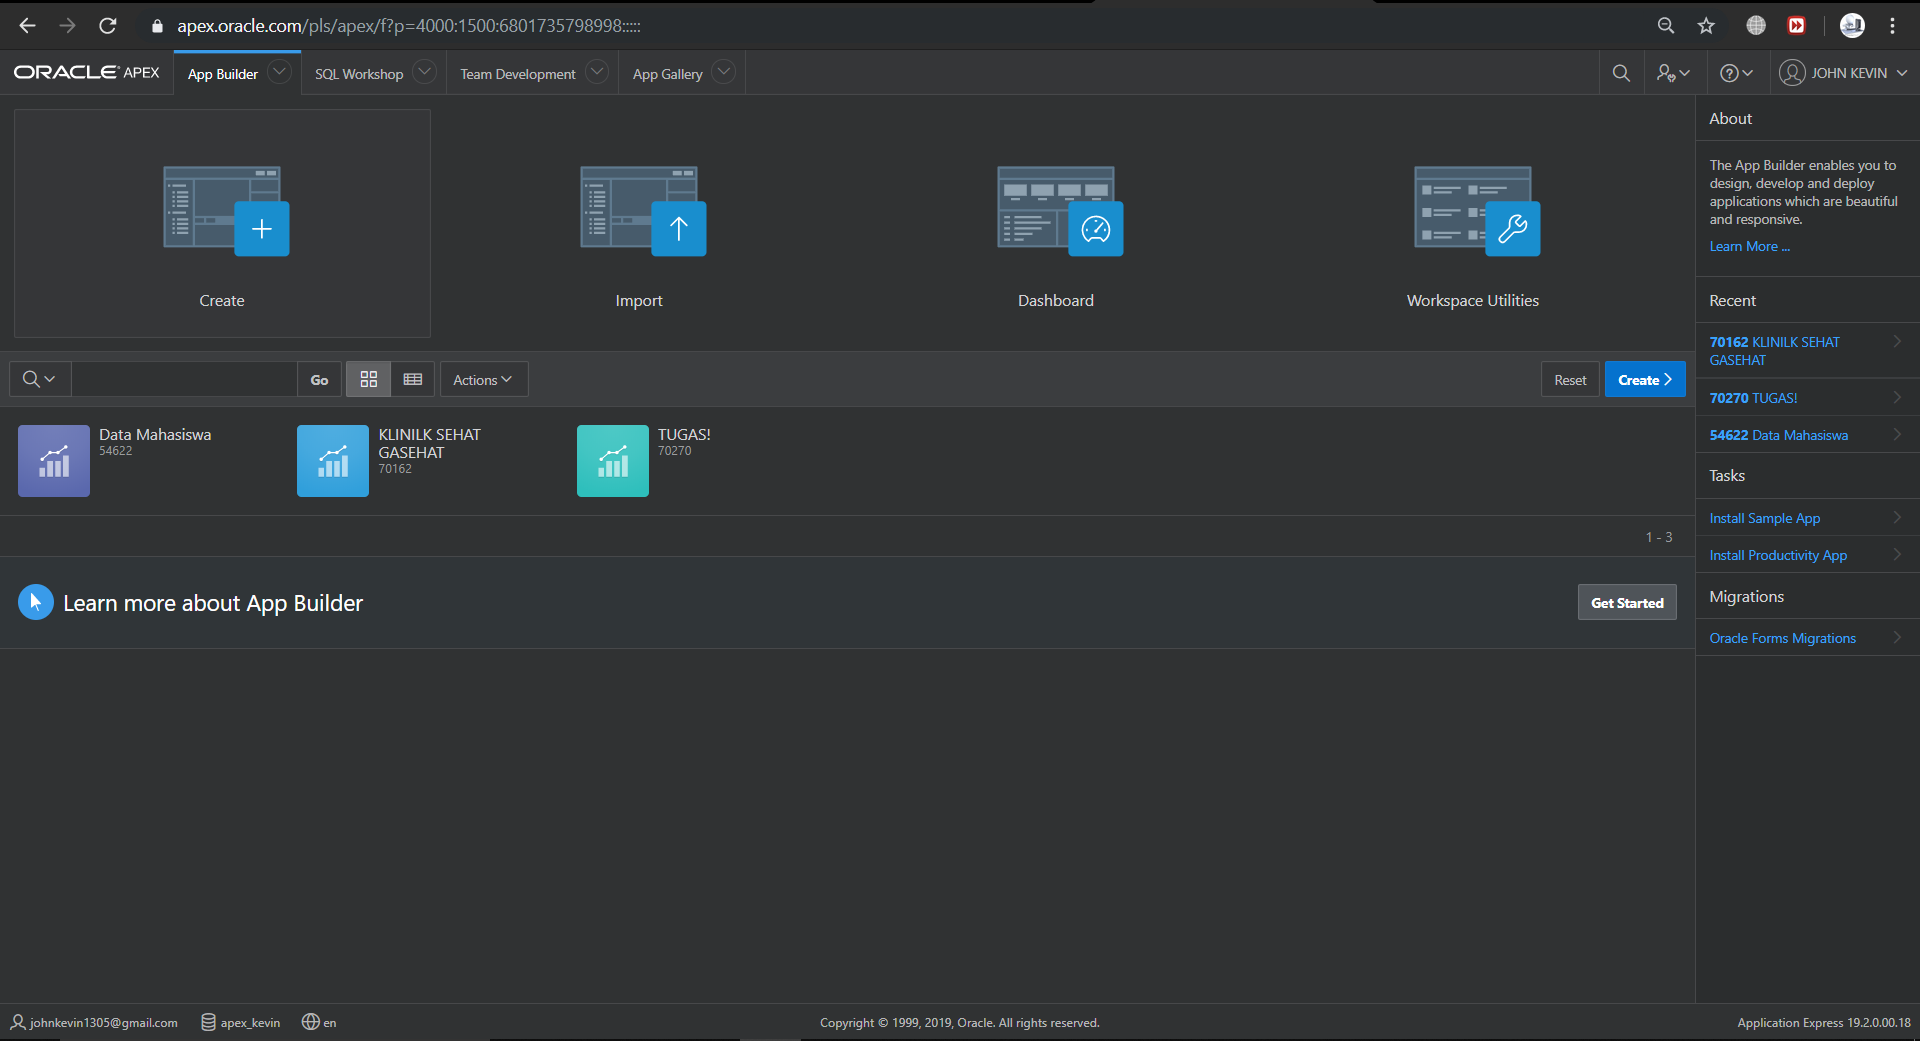
\includegraphics[width=7.5cm]{figure/C.png}
\caption{CREATE}
\end{center}
\end{figure}

\item Setelah itu pilih \textit{New Application}
\begin{figure}[h]
\begin{center}
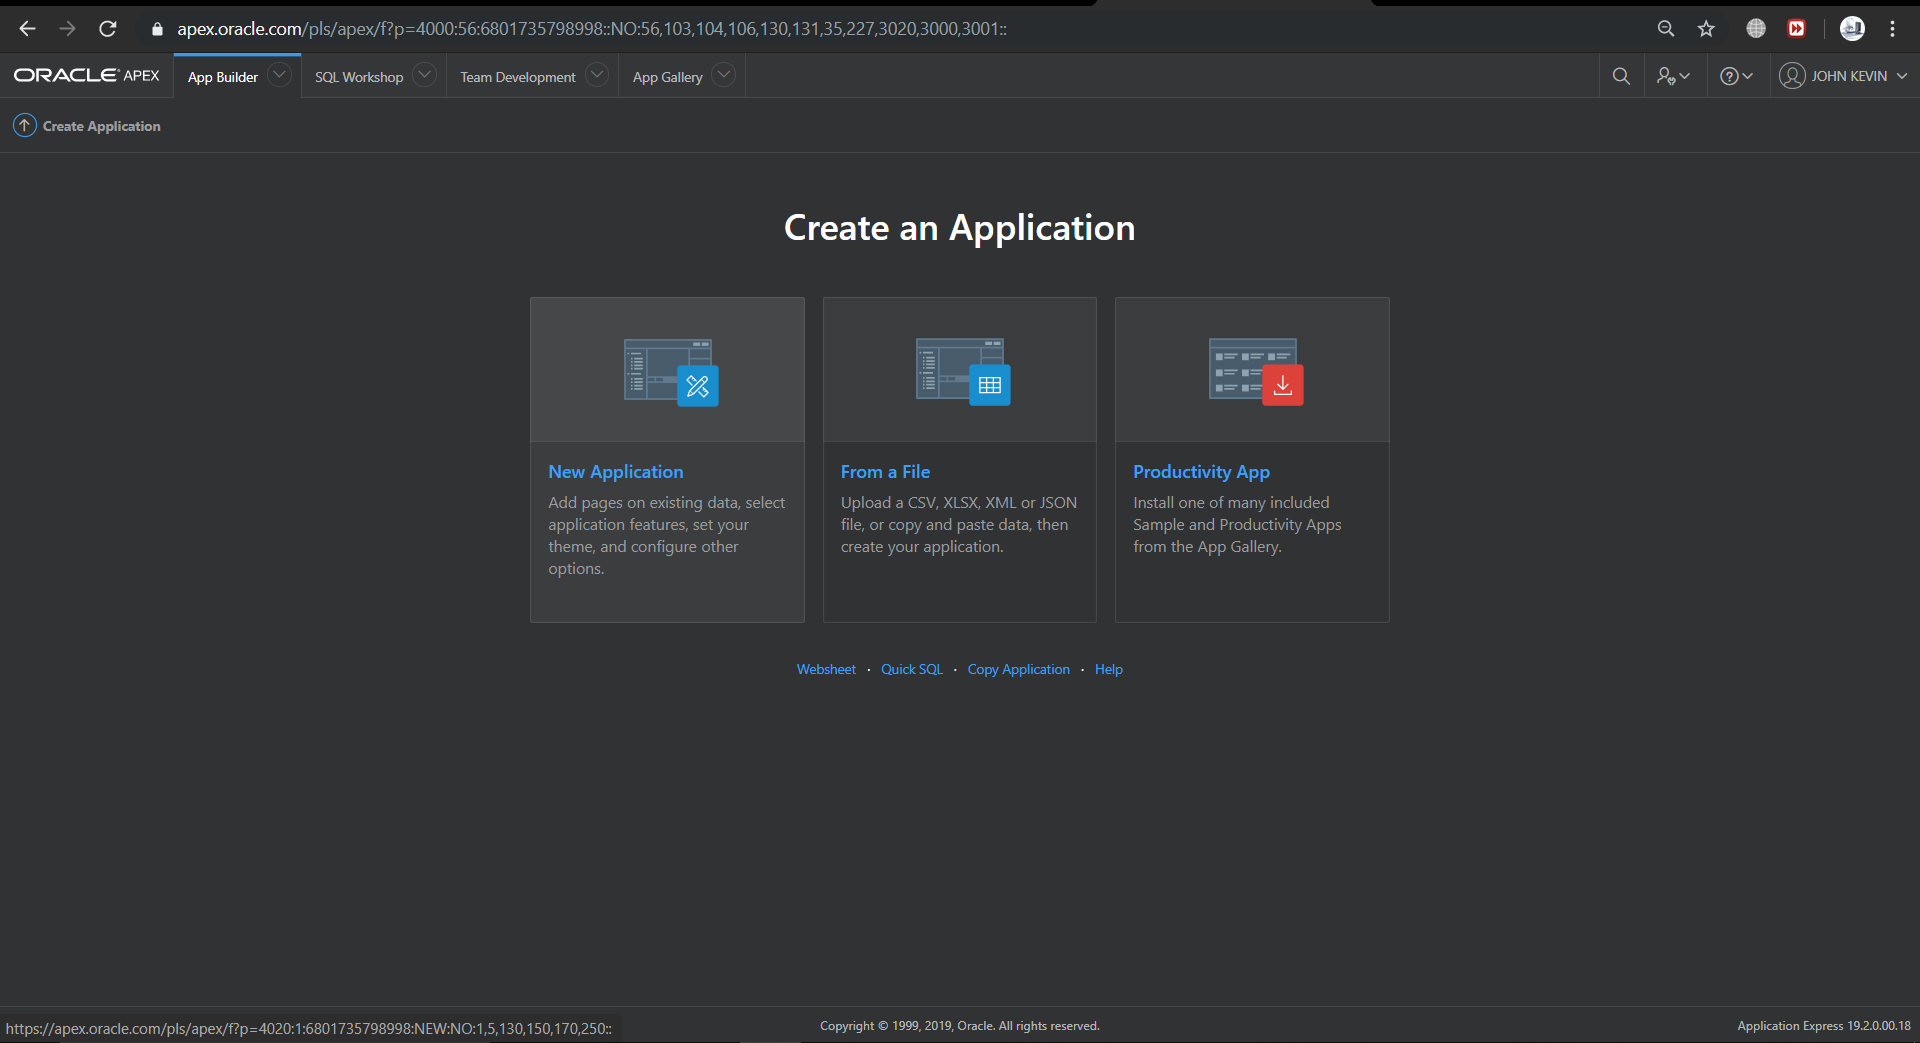
\includegraphics[width=7.5cm]{figure/NA.png}
\caption{NEW APPLICATION}
\end{center}
\end{figure}

\item Silahkan isi nama aplikasi yang diinginkan dan tampilan pada halaman tabel ingin seperti apa
\begin{figure}[h]
\begin{center}
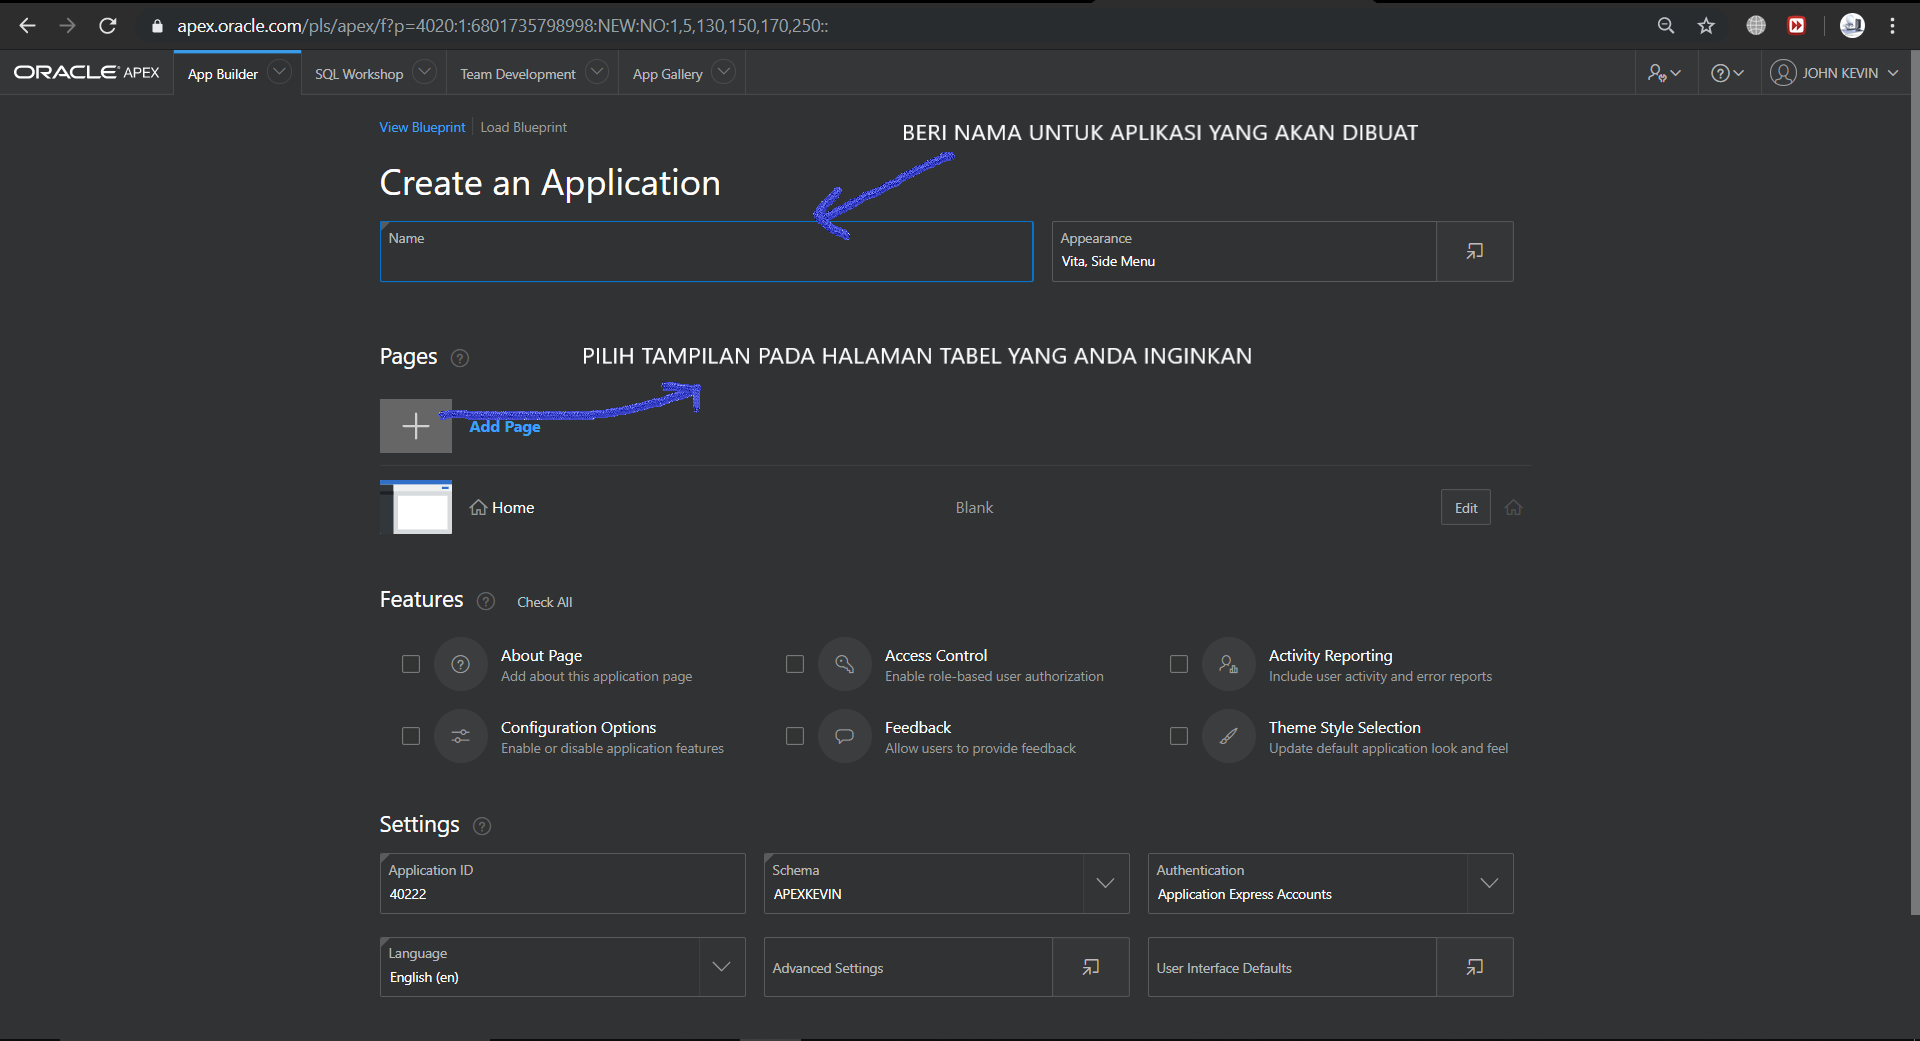
\includegraphics[width=10cm]{figure/CA1.png}
\caption{ISI NAMA DAN BENTUK TAMPILAN}
\end{center}
\end{figure}

\item Setelah nama aplikasi dan tampilan tabel telah anda tentukan selanjutnya silahkan pilih \textit{Create Application}
\begin{figure}[h]
\begin{center}
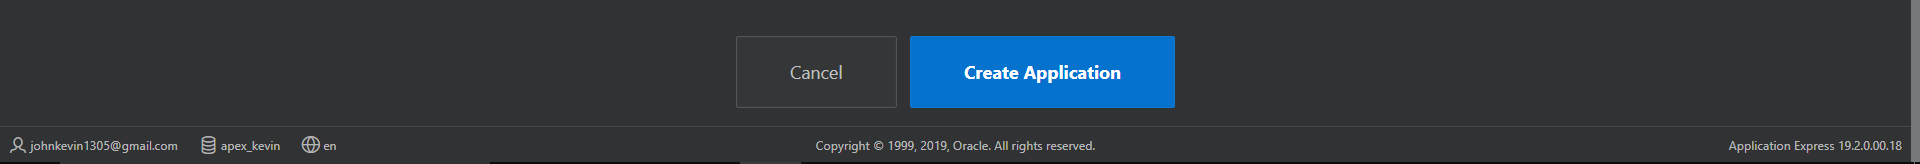
\includegraphics[width=12.5cm]{figure/CA2.png}
\caption{CREATE APPLICATION}
\end{center}
\end{figure}

\item Selanjutnya setelah aplikasi berhasil dibuat, anda dapat menjalankannya dengan cara memilih \textit{Run Application}
\begin{figure}[h]
\begin{center}
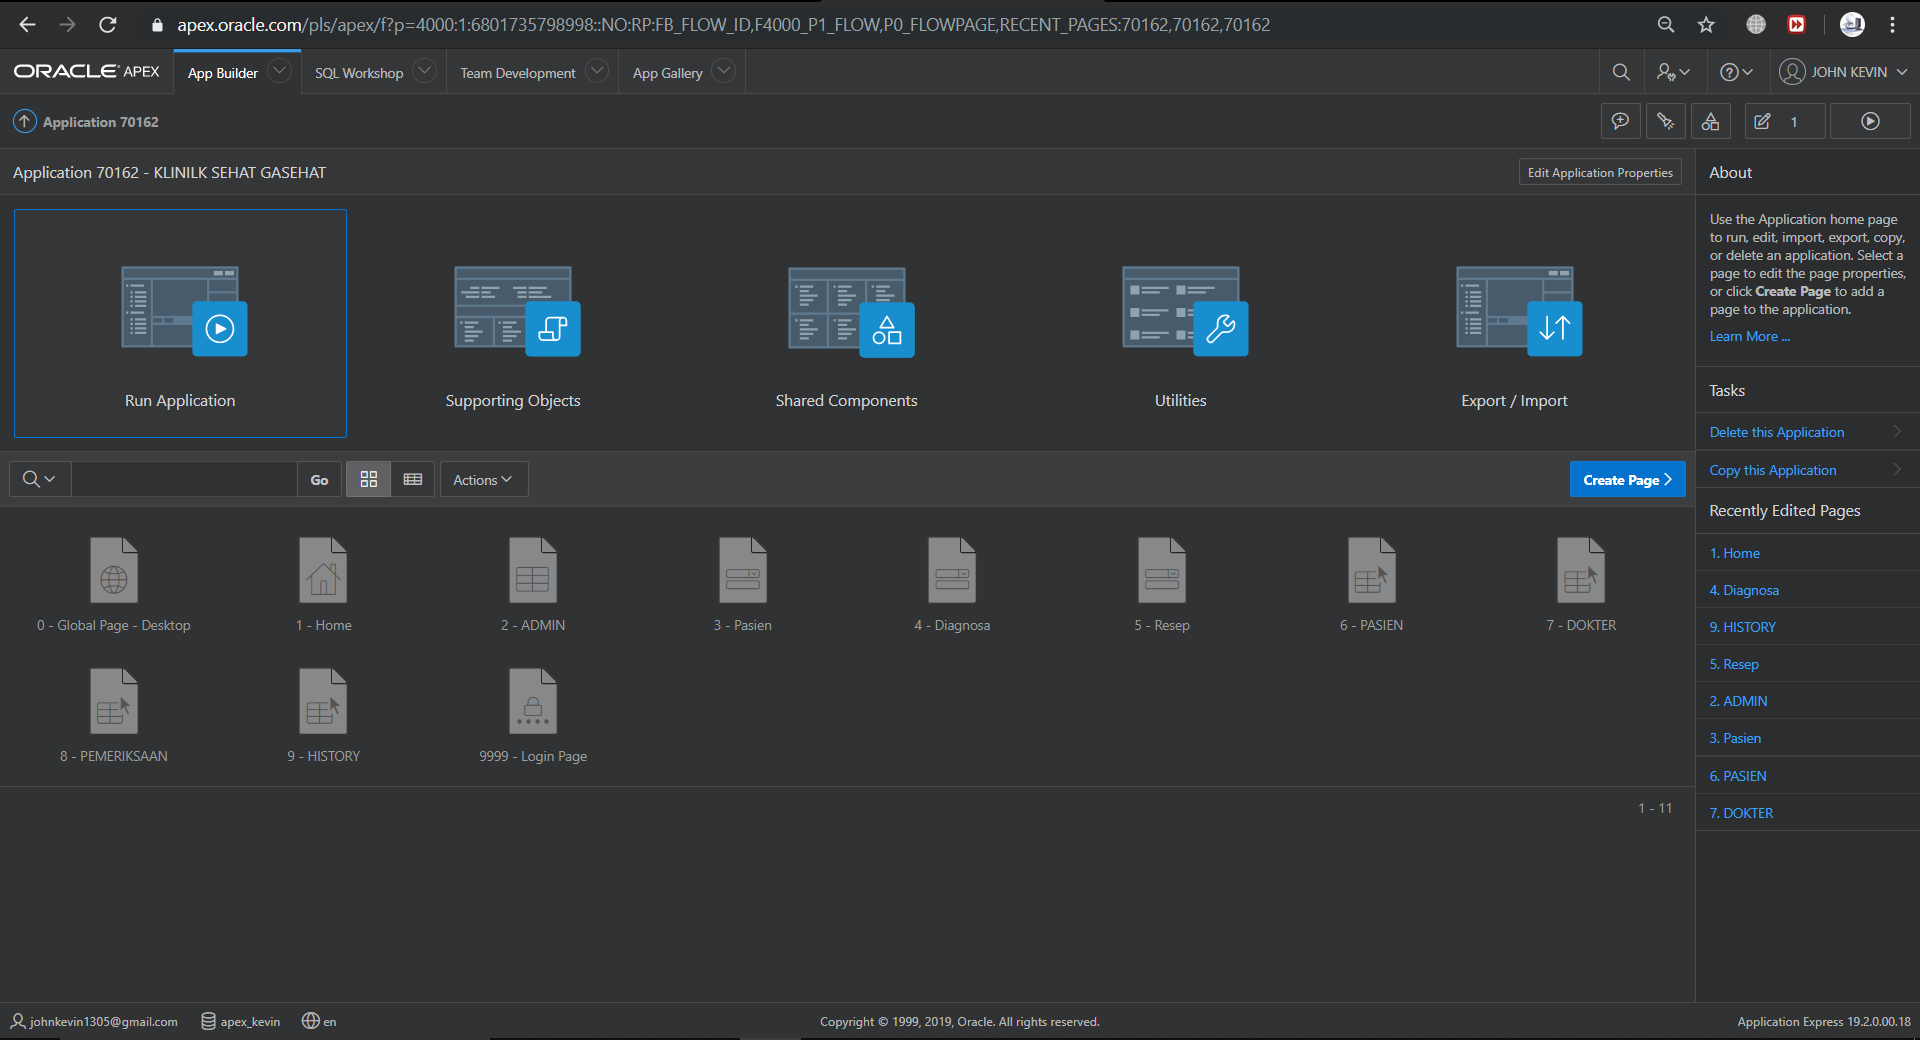
\includegraphics[width=11cm]{figure/RA.png}
\caption{MENUJU KE HALAMAN UTAMA}
\end{center}
\end{figure}

\item Setelah anda memilih \textit{Run Application}, akan muncul halaman \textit{login} untuk mengakses aplikasi yang telah dibuat. Anda dapat menggunakan \textit{Username} dan \textit{Password} pada saat anda masuk pada aplikasi \textit{Oracle Apex} anda.
\begin{figure}[h]
\begin{center}
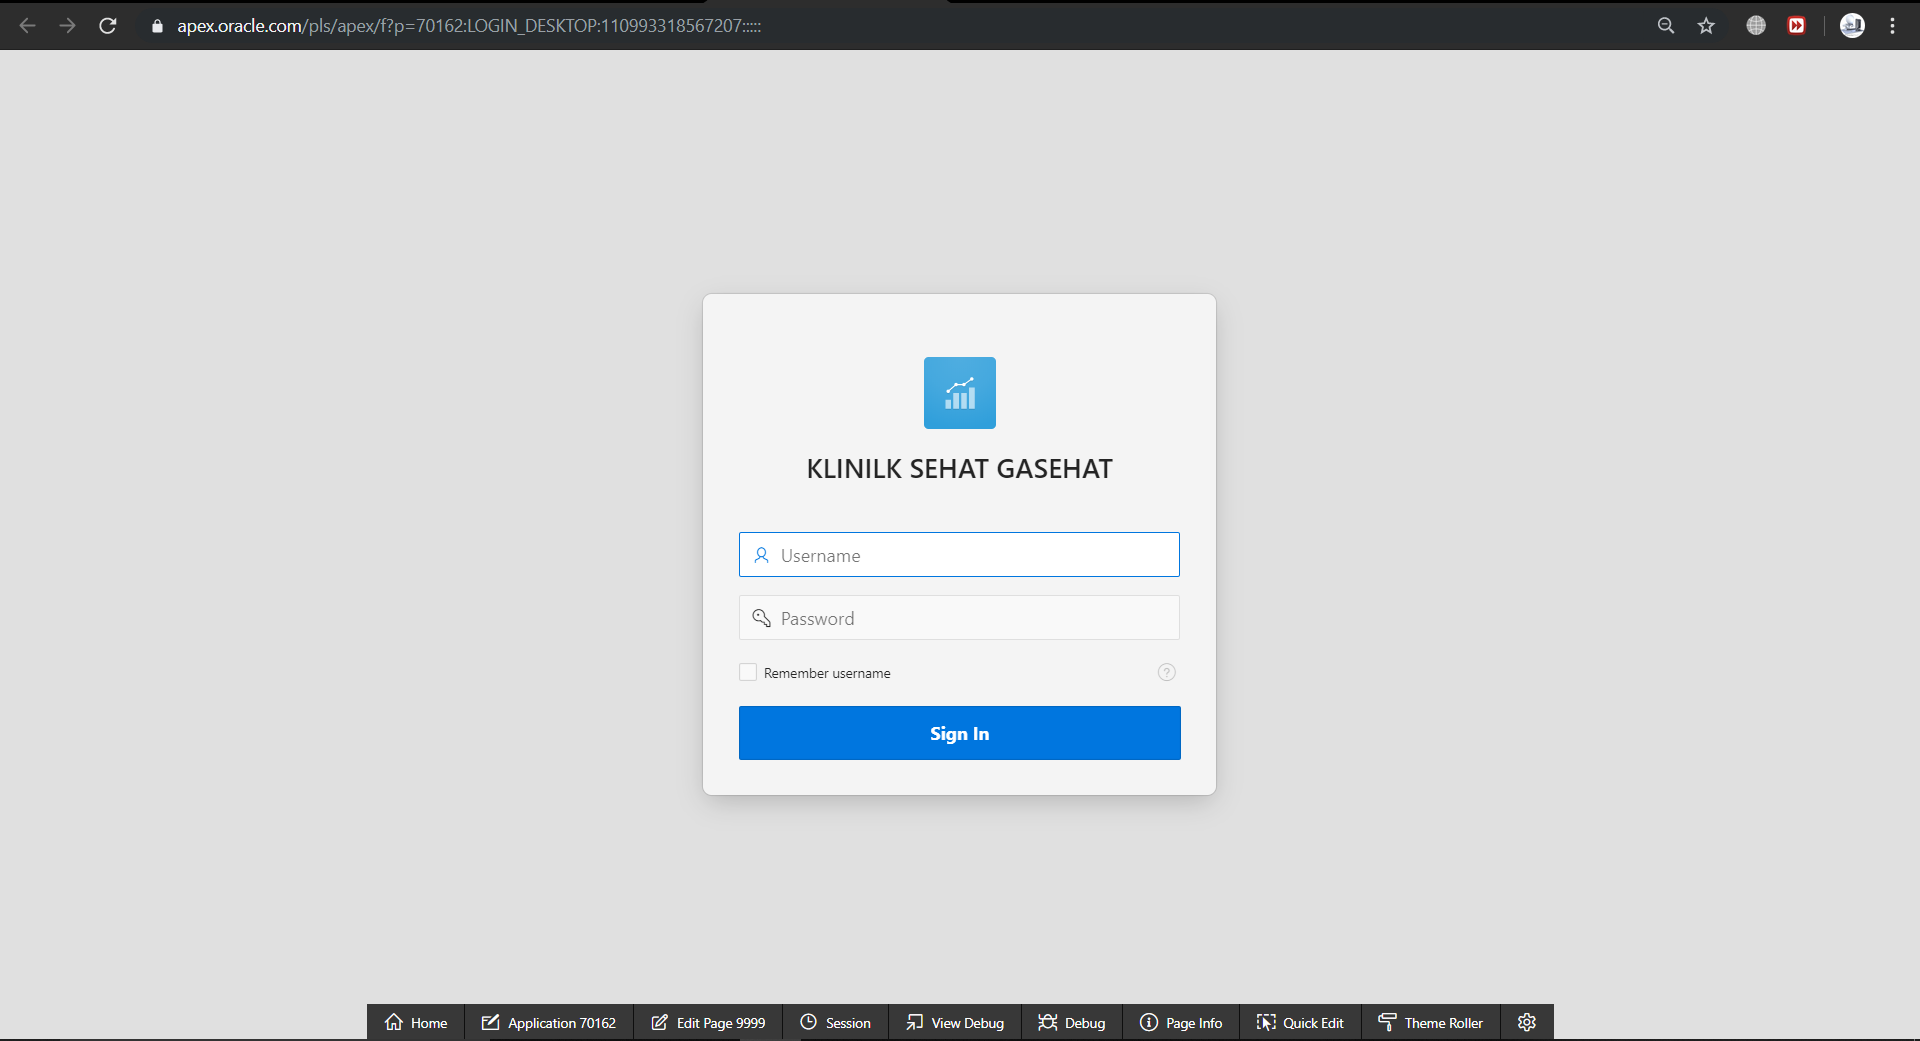
\includegraphics[width=8cm]{figure/L.png}
\caption{LOGIN APLIKASI}
\end{center}
\end{figure}

\item Setelah anda berhasil \textit{Login}, anda akan berada pada halaman utama aplikasi yang telah anda buat
\begin{figure}[h]
\begin{center}
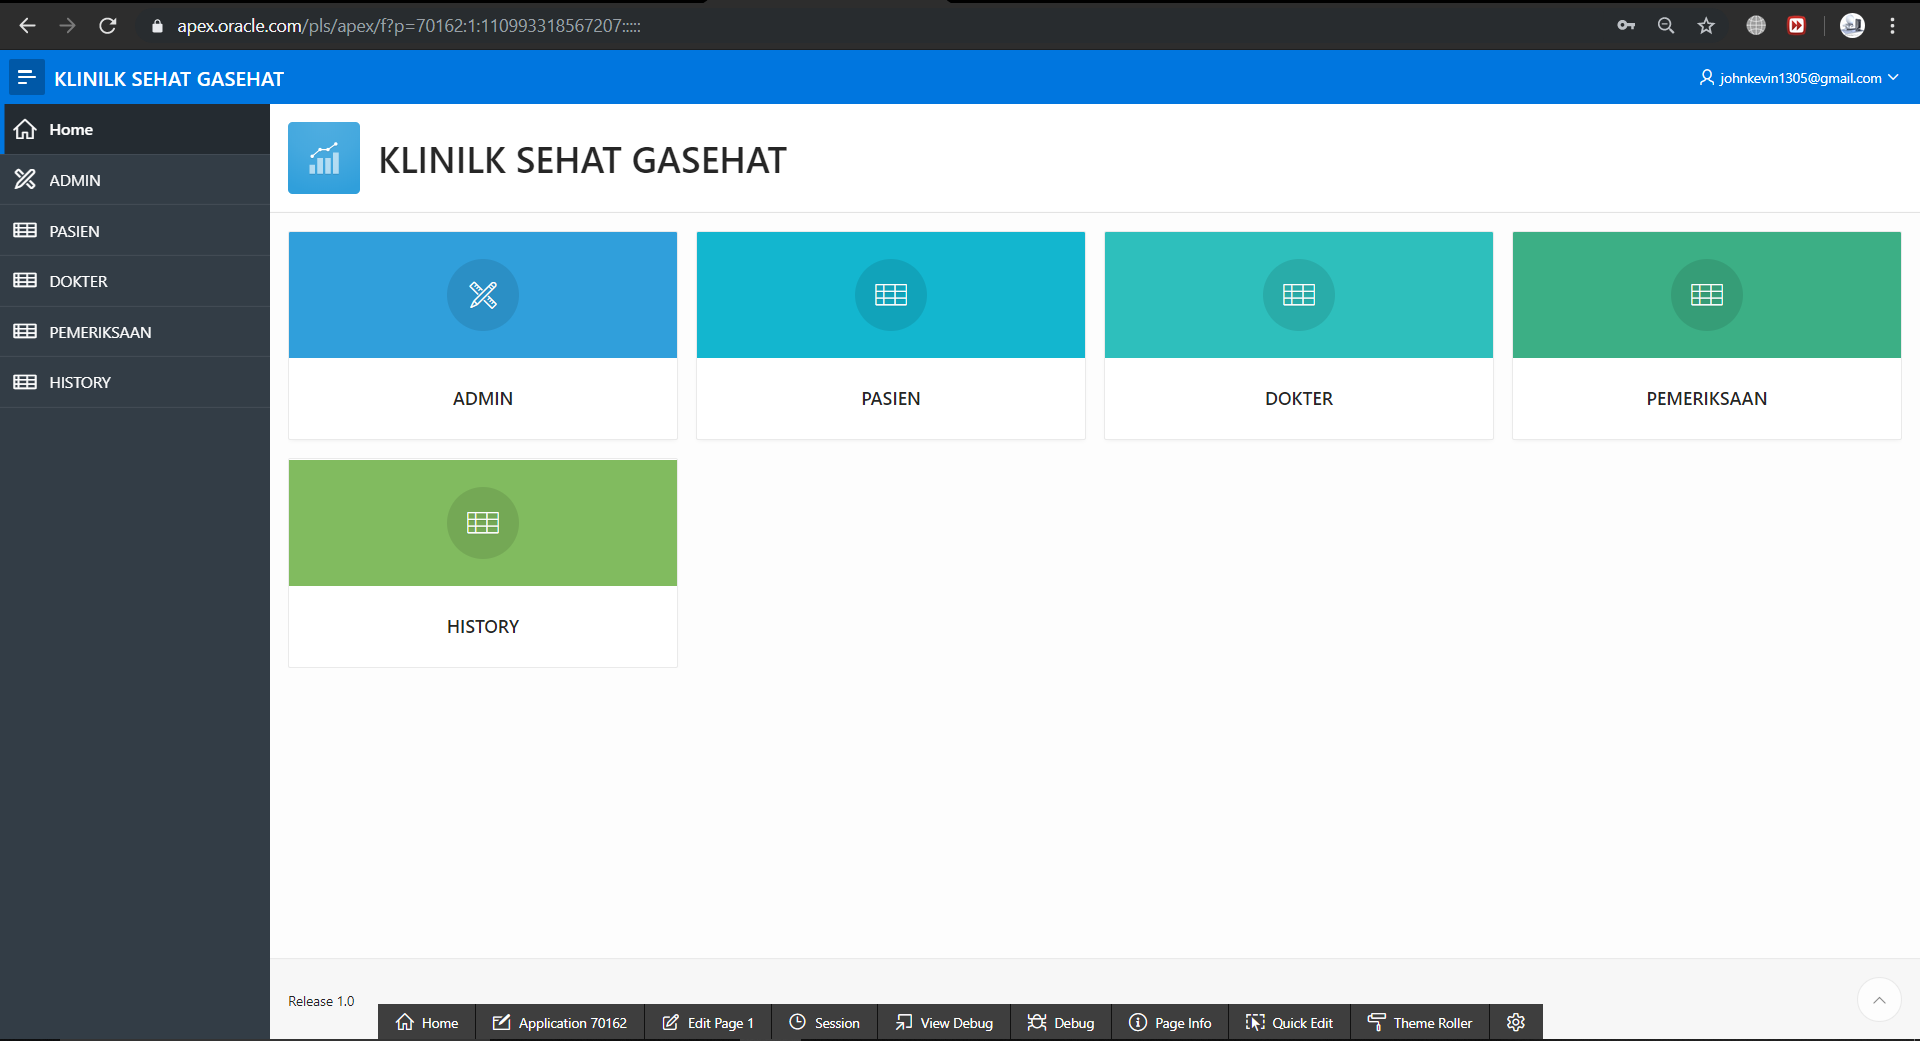
\includegraphics[width=8cm]{figure/H.png}
\caption{HALAMAN UTAMA APLIKASI}
\end{center}
\end{figure}
\end{enumerate}

\end{document}